%polar exemple
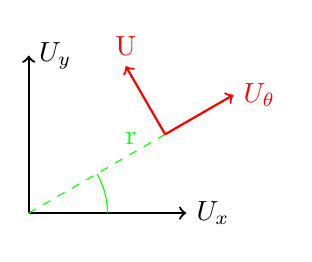
\begin{tikzpicture}
	\draw[thick, black, ->] (0, 0) -- (0, 2) node [right] {$U_y$};
	\draw[thick, black, ->] (0, 0) -- (2, 0) node [right] {$U_x$};
	\draw[dashed, green] (0, 0) --+ (30:3cm) node [midway, above] {r};
	\draw[red, thick, ->] (30:2cm) --+ (30:1cm) node [right] {$U_\theta$};
	\draw[red, thick, ->] (30:2cm) --+ (120:1cm) node [above] {U};
	\draw[green] (1, 0) arc (0:30:1cm);
\end{tikzpicture}

% Define the rings. Store them in macros to make things
% more flexible. 
\def\circleA{(0.5,0) circle (1)}
\def\circleB{(0,0) circle (1)}
\def\circleE{(0, 0) circle(0.5)}

\begin{tikzpicture}
	\draw[name path=circleA, red, thick, fill=gray, opacity=0.5] \circleA;
	\draw[name path=circleB, blue, thick, fill=gray, opacity=0.5] \circleB;
	\draw[black, name intersections={of=circleA and circleB, total=\t}, fill=black] \foreach \s in {1,...,\t}{(intersection-\s) circle (2pt)};
	\node at (0.25, -1) [below, rectangle, black, fill=gray] {$A \cup B$};
\end{tikzpicture}
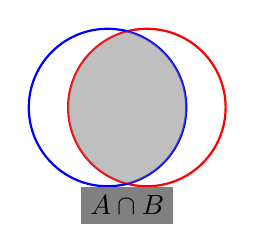
\begin{tikzpicture}
	\draw[red, thick] \circleA;
	\draw[blue, thick] \circleB;
	\begin{scope}
		\clip \circleA;
		\fill [gray, opacity=0.5] \circleB;
	\end{scope}
	\node at (0.25, -1) [below, rectangle, black, fill=gray] {$A \cap B$};
\end{tikzpicture}

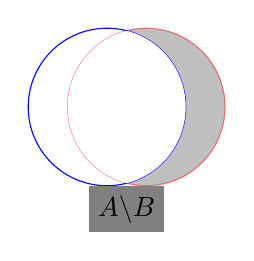
\begin{tikzpicture}
	\draw[red, fill=gray, opacity=0.5] \circleA;
	\draw[blue] \circleB;
	\begin{scope}
		\clip \circleA;
		\fill [white] \circleB;
	\end{scope}
	\node at (0.25, -1) [below, rectangle, black, fill=gray] {$A\backslash B$};
\end{tikzpicture}
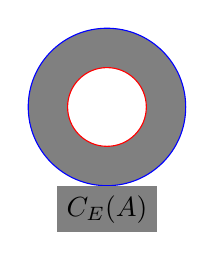
\begin{tikzpicture}
	\draw[blue, fill=gray] \circleB;
	\draw[red, fill=white] \circleE;
	\node at (0, -1) [below, rectangle, black, fill=gray] {$C_E(A)$};
\end{tikzpicture}

considérons la somme \[\sum_{k=1}^{n} a_k\]
\[(\vec{AB}, \vec{AC}) = Arg(\cfrac{Z_C-Z_A}{A_B - Z_A})\]

%Probability tree
\tikzstyle{level 1}=[level distance=3.5cm, sibling distance=3.5cm]
\tikzstyle{level 2}=[level distance=3.5cm, sibling distance=2cm]
\begin{tikzpicture}[grow=right, sloped]
	\node {Bag 1}
	child{
		node {Bag2}
		child{
			node {text}
			edge from parent
			node [below] {$\frac{1}{4}$}
		}
		edge from parent
		node[below]{$\frac{3}{4}$}
		node[above]{D}
	}
	child{
		node {Bag2}
		child{
			node {text}
			edge from parent
			node [below] {$\frac{1}{4}$}
		}
		edge from parent
		node[below]{$\frac{3}{4}$}
		node[above]{D}
	};

\end{tikzpicture}

%dirtree exemple (like trees for folders)
\begin{tikzpicture}[dirtree]
\node {toplevel} 
    child { node {Foo}
            child { node {foo} }
            child { node {bar} }
            child { node {baz}
				child { node {bar} }}
    }
    child { node {Bar}
        child { node {foo} }
        child { node {foo} }
        child { node {foo} }
        child { node {foo} }
        child { node {bar} }
        child { node {baz} }
    }
    child { node {Baz}
        child { node {foo} }
        child { node {bar} }
        child { node {baz} }
    };
\end{tikzpicture}

%Table of variations
\begin{tikzpicture}
	\tkzTabInit{$x$/1,$f'(x)$/1,$f(x)$/2}{$0$, $1$, $e$}
	\tkzTabLine{d,-,z,+}
	\tkzTabVar{D+/$1$,-/$0$,+/$3$}
	\tkzTabVal{1}{2}{0.5}{$0.5$}{$0.5$}
\end{tikzpicture}

\begin{tikzpicture}
	\tkzTab{$x$/1,$f'(x)$/1,$f(x)$/2}{$0$, $1$, $e$}{d,-,z,+}{D+/$1$,-/$0$,+/$3$}
	\tkzTabVal[draw]{1}{2}{0.5}{$0.5$}{$0.7$}
\end{tikzpicture}
